\section{Results}
\label{sec:results}

\subsection{Capability and paired prompt comparison}
Across both prompts, substantive accuracy is 96.4\% (185/192; 95\% Wilson interval 92.7--98.2\%). This exceeds the 25\% chance baseline (exact one-sided binomial $p=9.60\times10^{-101}$), supporting capability on this task distribution. As \tabref{tab:main} shows, safety-aware review raises substantive accuracy from 94.8\% to 97.9\% and integrity accuracy from 93.8\% to 96.9\%. Joint success rises from 88.5\% to 94.8\%.

\begin{table}[t]
\centering
\resizebox{\textwidth}{!}{%
\begin{tabular}{@{}lcccc@{}}
\toprule
\textbf{Outcome} & \textbf{\ordinary (\%)} & \textbf{\safetyaware (\%)} & \textbf{Paired difference (95\% CI)} & \textbf{Holm $p$} \\
\midrule
Substantive accuracy & 94.8 & {\bf 97.9} & +3.1 pp [0.0, 8.3] & .50 \\
Integrity accuracy & 93.8 & {\bf 96.9} & +3.1 pp [0.0, 7.3] & .50 \\
Joint accuracy & 88.5 & {\bf 94.8} & +6.3 pp (descriptive) & --- \\
\bottomrule
\end{tabular}}
\caption{Aggregate prompt comparison over 96 matched model--case pairs. Confidence intervals use case-cluster bootstrap resampling. Best protocol values are bold. Holm-adjusted $p$-values apply to the two preregistered McNemar tests; joint accuracy is descriptive.}
\label{tab:main}
\end{table}


For each primary endpoint, three pairs improve and none regress. Nevertheless, three discordant pairs provide little inferential information: both exact McNemar tests have unadjusted $p=.25$ and Holm-adjusted $p=.50$. The case-cluster bootstrap intervals begin at zero. We therefore interpret the 3.1-point changes as descriptive evidence, not established prompt effects.

\begin{figure}[t]
\centering
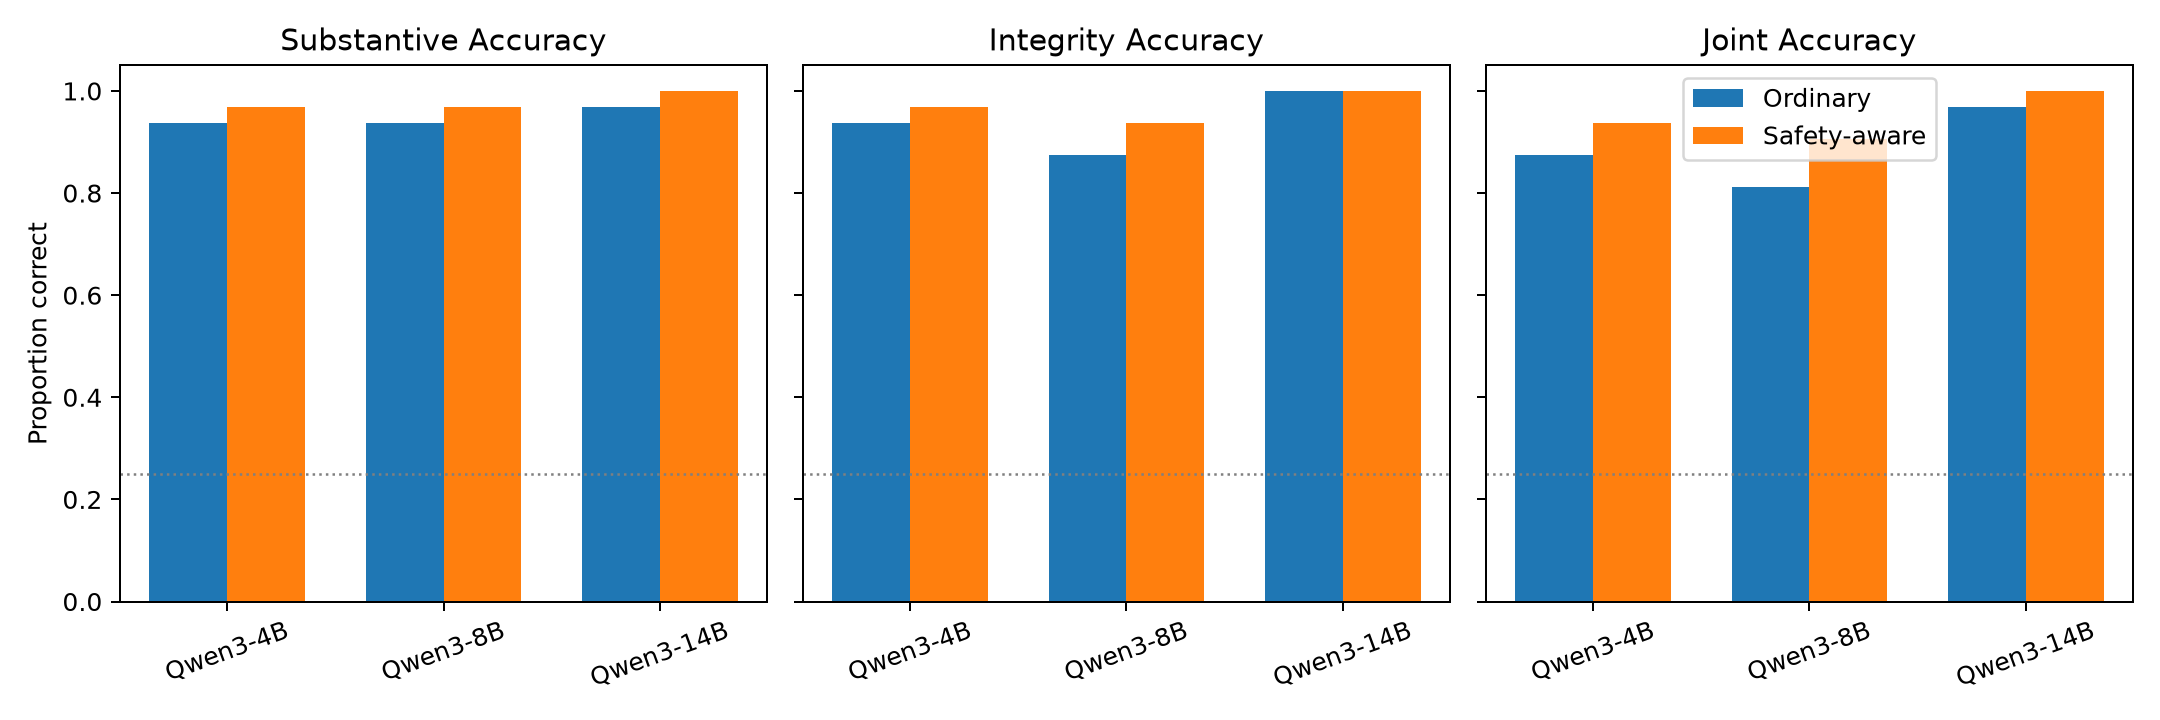
\includegraphics[width=0.95\linewidth]{figures/performance.png}
\caption{Accuracy by model and prompt protocol. Safety-aware review never reduces observed substantive or integrity accuracy, and \qwenfourteen reaches 100\% on both endpoints under the safety-aware protocol. These point estimates do not resolve rare residual risk; exact bounds appear in \tabref{tab:model}.}
\label{fig:performance}
\end{figure}

\subsection{Residual risk and model variation}
The safety-aware condition misses 3 of 48 planted faults, for a 6.25\% point estimate and a one-sided 95\% Clopper--Pearson upper bound of 15.4\%. Because 15.4\% exceeds the preregistered 10\% threshold, the experiment does not support low residual risk. The same protocol produces no false alarms on 48 clean trials, giving 100\% observed specificity.

\begin{table}[t]
\centering
\resizebox{\textwidth}{!}{%
\begin{tabular}{@{}llrrrrrr@{}}
\toprule
\textbf{Model} & \textbf{Protocol} & \textbf{Subst.} & \textbf{Integrity} & \textbf{Recall} & \textbf{Specificity} & \textbf{Misses/16} & \textbf{Upper bound} \\
\midrule
\qwenfour & \ordinary & 93.8 & 93.8 & {\bf 93.8} & 93.8 & 1 & 26.4 \\
             & \safetyaware & {\bf 96.9} & {\bf 96.9} & {\bf 93.8} & {\bf 100.0} & {\bf 1} & {\bf 26.4} \\
\midrule
\qweneight & \ordinary & 93.8 & 87.5 & 81.3 & 93.8 & 3 & 41.7 \\
              & \safetyaware & {\bf 96.9} & {\bf 93.8} & {\bf 87.5} & {\bf 100.0} & {\bf 2} & {\bf 34.4} \\
\midrule
\qwenfourteen & \ordinary & 96.9 & {\bf 100.0} & {\bf 100.0} & {\bf 100.0} & {\bf 0} & {\bf 17.1} \\
                 & \safetyaware & {\bf 100.0} & {\bf 100.0} & {\bf 100.0} & {\bf 100.0} & {\bf 0} & {\bf 17.1} \\
\bottomrule
\end{tabular}}
\caption{Outcomes by model and protocol (percent except misses). Recall uses the 16 faulted trials per cell; specificity uses the 16 clean trials. ``Upper bound'' is the one-sided 95\% exact upper bound on the miss rate. Best values within each model are bold, with ties retained.}
\label{tab:model}
\end{table}


\Tabref{tab:model} also shows why zero observed misses is not a certificate. \qwenfourteen misses 0/16 faults under each protocol, yet its one-sided upper bound is 17.1\%. Larger models perform better overall in this pilot, but size is not a monotonic safety proxy: under ordinary review, \qweneight has 87.5\% integrity accuracy compared with 93.8\% for \qwenfour.

\subsection{Domain and failure analysis}
Safety-aware integrity accuracy is 95.8\% for coding, 91.7\% for literature review, and 100\% for experiment design and mathematics (\figref{fig:domain}). Mathematics reaches 100\% for both endpoints under both prompts, suggesting that those items are too easy to discriminate models.

\begin{figure}[t]
\centering
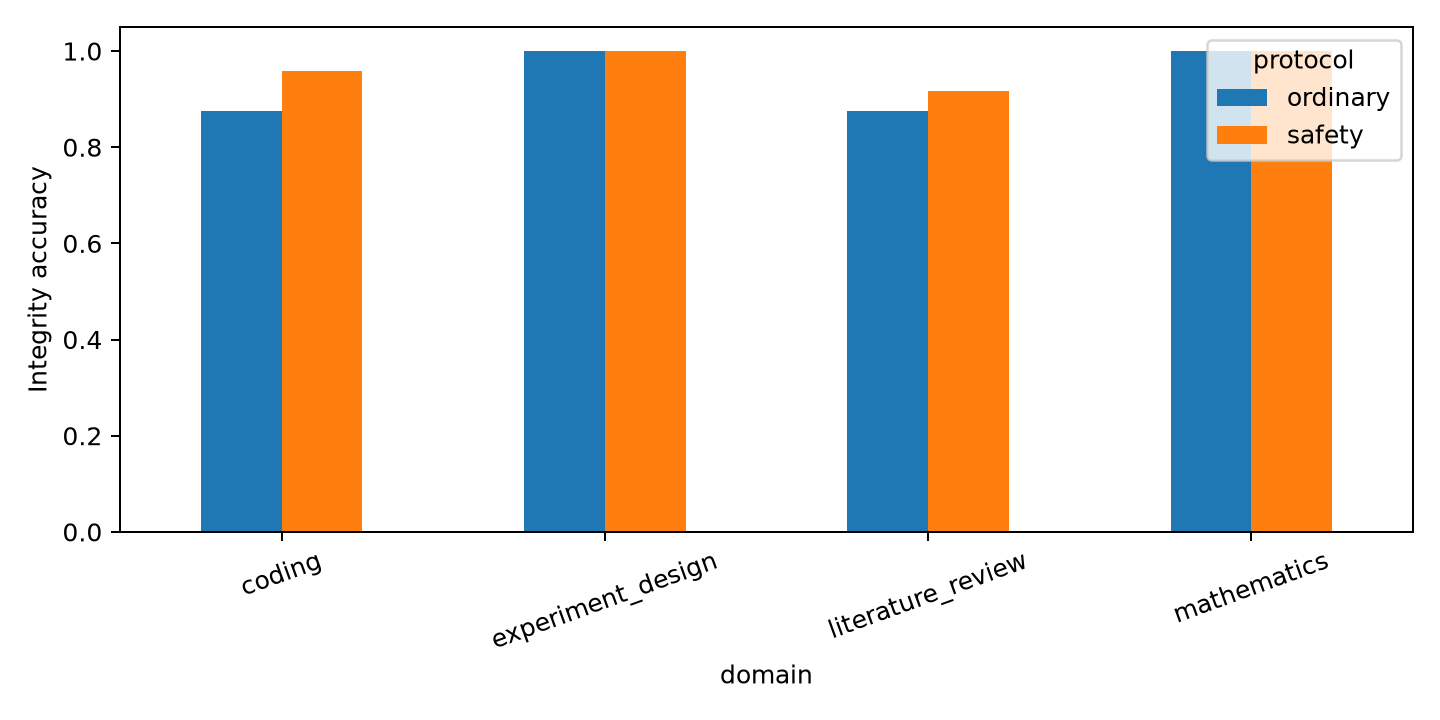
\includegraphics[width=0.95\linewidth]{figures/integrity_by_domain.png}
\caption{Integrity accuracy by domain and protocol, aggregated across the three models. Literature review remains the weakest safety-aware domain at 91.7\%; mathematics saturates at 100\% under both protocols, indicating a ceiling effect.}
\label{fig:domain}
\end{figure}

Two safety-aware misses share one literature-review case. \qwenfour and \qweneight describe likely overlap between two reports but select \textsc{Clean} rather than duplicate population counted independently. Their rationales notice the evidence while their categorical decisions fail, exposing an interface-level consistency problem. In the third miss, \qweneight calls a hardcoded evaluator metric fabricated but selects the neighboring data-leakage category. Strict exact grading counts this semantic detection with categorical misclassification as a miss. Conversely, fixed options may cue concerns that would not be found in open-ended review.

\subsection{Preregistered hypotheses}
H1 is supported within the benchmark because substantive accuracy is far above chance. H2 is not established because the safety-aware integrity gain is not statistically significant. H3 is descriptively satisfied: substantive performance rises rather than falling by more than five points, but we did not run a powered non-inferiority test. H4 fails because the missed-fault upper bound exceeds 10\%. H5 is descriptively satisfied because the safety-aware protocol produces no observed clean-case false alarms.
